% Chapter Template

\chapter{Data Mining} % Main chapter title

\label{Chapter1} % Change X to a consecutive number; for referencing this chapter elsewhere, use \ref{ChapterX}

%----------------------------------------------------------------------------------------
%	SECTION 1
%----------------------------------------------------------------------------------------

%-----------------------------------
%	SUBSECTION 1
%-----------------------------------
\section{Informatia inseamna putere}
In ziua de azi, datorita serviciilor ieftine de stocare a datelor, stocarea de informatii devine o treaba usoara si deschide calea invatarii unor lucruri noi. Asadar obtinerea de noi cunostine se transforma in serviciul de extragere prin diferite metode de noi idei  dintr-un ocean de informatii stocate care asteapta sa fie analizate. In zilele noastre majoritea actiunilor cotidiene sunt inregistrate si stocate. Datorita numarului mare de oameni si de actiuni pe care un om le face se transmit date intr-un volum greu de imaginat. Avand disponibil un volum atat de imens de date partea mai grea devine analiza, invatarea si corelarea acestora. Desi lucrul cu date a fost folosit de mult timp de catre economisti, statisticieni sau meteorologi e de remarcat cresterea recenta al oportunitatilor de gasire al modelelor in date. Bazat pe \parencite{DMP2011} numarul datelor la nivel global stocat in bazele de date se dubleaza la fiecare 20 de luni. Avand in vedere volumul imens de date cu care suntem inundati si eficientizarea calculatoarelor de a suporta cautari are ca urmare cresterea interesului in data mining. Astfel, data mining, reprezinta o solutie la a gasi noi concepte, noi idei care pot ajuta la rezolvarea unor probleme din diferite ramuri, de exemplu, intr-un context comercial, obtinandu-se un avantaj comercial. 

%-----------------------------------
%	SUBSECTION 2
%-----------------------------------
\section{Definitie}
Data mining reprezinta procesul de analiza si cercetare asupra unui volum imens de date stocat in baze de date sau alte tipuri de stocare de informatii. Procesul are ca scop descoperirea de noi cunostinte precum: modele, asocieri, comportamente, anomalii, structuri semnificative care sa ofere descoperiri noi, inovatoare. Procesul poate fi privit ca o cutie inchisa care produce rezultatul dorit. La fel cum si \parencite{Disco} precizeaza, procesul de data mining poate avea si rezultate nedorite daca o metoda este aplicata intr-un context nepotrivit sau modelele sunt construite pe presupuneri eronate.   

%-----------------------------------
%	SUBSECTION 3
%-----------------------------------
\section{CISP}
"Cross-industry standard practice"(CISP) reprezinta un proces standard de abordare al solutiilor de tip data mining. Acest standard a fost creat cu scopul de a fi liber si de a fi utilizat de catre toti cei care folosesc data mining pentru a rezolva diferite probleme. A fost creat, cumva natural, datorita faptului ca fiecare incerca sa isi fac propriul proces, astfel creandu-se haos. Asadar, CISP, a luat nastere ca fiind un standard care nu e specific unei industrii, aplicatii, sau unui tool. Bazat pe standardul CISP, un proiect de tip data mining consta din 6 etape dupa cum se poate vedea si din Figure~\ref{fig:CISP}. 
\begin{figure}[th]
\centering
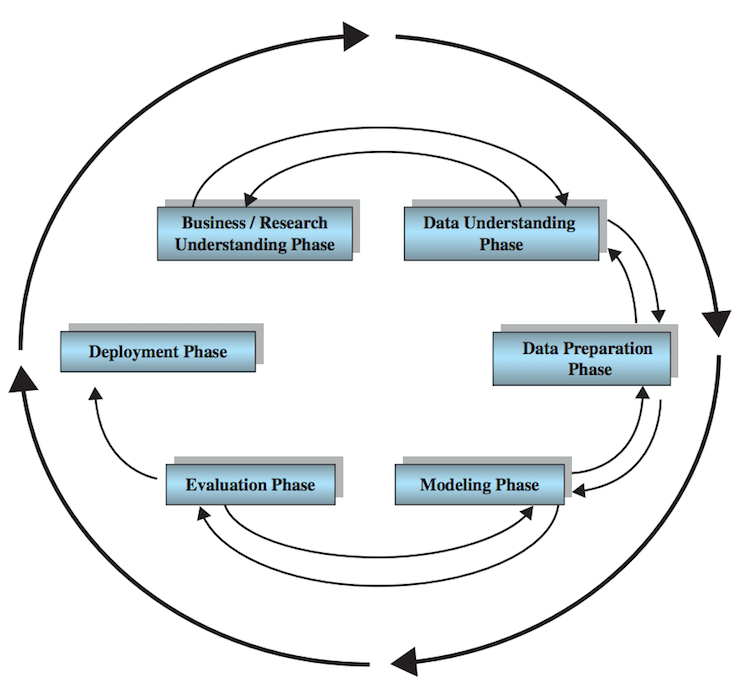
\includegraphics{Figures/CISP}
\decoRule
\caption[CISP]{CISP}
\label{fig:CISP}
\end{figure}
Procesul definit e unul iterativ care se poate adapta; fiecare componenta depinde de componenta precedenta iar in caz de iregularitati procesul se poate intoarce inapoi la pasul precedent.
% %-----------------------------------
% %	SUBSECTION 3_1
% %-----------------------------------
% \subsection{CISP}

% Data mining poate fi asociat cu expresii precum descoperirea de cunostinte in baze de date, (potrivit lui \parencite{JiaweiIntro}), cu toate ca alti cercetatoti considera, data mining, ca fiind un pas important in descopeirirea de noi cunostinte. Se poate sintetiza procesul de descoperire a cunostintile din date in urmatorii pasi (bazat pe \parencite{JiaweiIntro}): curatarea datelor, integrarea datelor, selectarea datelor, transformarea datelor, extragerea datelor, evaluarea modelelor si prezentarea cunostintelor. Acesti 7 pasi pot fi impartiti in 2 grupuri mai mari. Primii 4 pasi pot fi priviti ca construirea unor depozite de date si efectuare unor operatii pe acestea. Ultimii 3 pasi se transforma intr-un proces iterativ denumit data mining.  

%-----------------------------------
%	SUBSECTION 4
%-----------------------------------
\section{La ce se foloseste?}

Cerintele in care data mining e folosit s-au grupat in 6 clase (potrivit cu \parencite{Disco}).
\begin{itemize}
\item Descrierea: reprezinta modul prin care se cauta cai care precizeaza unele "trenduri" sau modele care se observa in date.
\item Estimarea: se refera la a estima valoarea numerica a unui atribut tinta avand la dispozitie variabile predictorii care pot fi de tipul numerice sau categoriale(?). De exemplu se pot face estimari despre cat v-a cheltui o familie cu 2 copii pentru inceperea unui nou an scolar. De asemenea, un alt exemplu il reprezinta prezenta la vot pentru alegerile curente ale cetatenilor cu varsta cuprinsa intre [18-24] cu drept de vot bazat pe alegerile din anii trecuti.
\item Predictia: este similara cu estimarea si clasificarea cu precizarea ca rezultatul predictiei o sa se intample in viitor. Exemple de predictii ar fi: pretul unei actiuni la bursa peste cateva luni sau cine va castiga campionatul mondial de fotbal. Bazat pe \parencite{Disco}, in alegerile prezidentiale din America din 2012, echipa de campanie a lui Barack Obama s-a folosit de data mining. Acestia au folosit data mining pentru a identifica tipul sustinatorilor lui Barack Obama si s-au asigurat ca acestia merg la vot si au mai folosit pentru a face predictii despre voturile pentru Barack Obama in fiecare judet. Un exemplu de predictie pentru judetul Hamilton din statul Ohio considerat "indecis", a fost de 56.4\% iar rezulultul final a fost de 56.6\%.
\item Clasificarea: este asemantoare cu estimarea cu diferenta ca variabila tinta, care se doreste sa fie clasificata, are ca valori categorii. Modelul de data mining examineaza datele care contini valori pentru atributele predictorii si atributul tinta.
\item Gruparea: se refera la procesul de a grupa date, observatii, cazuri in clase asemanatoare. O grupare reprezinta o colectie de obiecte care prezinta insusiri asemanatoare intre ele. Gruparea reprezinta o sarcina diferita conceptual fata de clasificare, estimare sau predictia. In procesul de grupare nu exista un atribut tinta care sa fie clasificat. In schimb, gruparea, incearca sa imparta datele in grupuri sau clase relativ omogene, astfel incat similaritatiile elementelor dintr-un grup sunt maximizate iar disimilaritatille cu elemente straine grupului sunt minimizate.
\item Asocierea: consta in a determina ce atribute "merg impreuna". Are ca scop gasirea de legaturi intre atribute. Este folosita cu succes in analiza pietei cumparatorilor din magazine pentru a gasi ce produse sunt cumparate impreuna si ce produce nu sunt. Asocierile sunt de forma "daca antecedentul atunci consecinta".
\end{itemize}
